% Metódy inžinierskej práce

\documentclass[10pt,twoside,slovak,a4paper]{article}

\usepackage[slovak]{babel}
\usepackage[IL2]{fontenc} % lepšia sadzba písmena Ľ než v T1
\usepackage[utf8]{inputenc}
\usepackage{graphicx}
\usepackage{url} % príkaz \url na formátovanie URL
\usepackage{hyperref} % odkazy v texte budú aktívne (pri niektorých triedach dokumentov spôsobuje posun textu)
\usepackage{marvosym} % symbol EUR

\usepackage{cite}
%\usepackage{times}

\pagestyle{headings}

\title{Extrakcia informácii z webu pre analýzu dát pomocou Python\thanks{Semestrálny projekt v predmete Metódy inžinierskej práce, ak. rok 2023/24, vedenie: Ing. Mohammad Yusuf Momand, MSc.}} % meno a priezvisko vyučujúceho na cvičeniach

\author{Štefan Kučerák\\[2pt]
	{\small Slovenská technická univerzita v Bratislave}\\
	{\small Fakulta informatiky a informačných technológií}\\
	{\small \texttt{xkucerak@stuba.sk}}
	}

\date{\small 16. december 2023}



\begin{document}

\maketitle
%Čím sa zaoberáte a prečo (ako to definujú iní a ako by ste to definovali vy)?
%Aký je stav v oblasti (s odkazmi na zdroje)?
%Čo pokladáte za významný problém v tejto oblasti a prečo (opora v literatúre)?
%Je nejaké riešenie a aké?
%Je vaše riešenie podobné iným (hoci aj z inej oblasti a len v z určitého hľadiska)?
%O čom je článok, k čomu ste ním prispeli a čo zostáva otvorené?


\begin{abstract}
Problém nastáva pri získavaní veľkého množstva dát z prostredia otvoreného webu. Vykonávanie tejto činnosti ľuďmi by bolo veľmi časovo náročné. Riešením tohto problému je proces, ktorý je v angličtine označovaný ako "Web scraping". Je to spôsob extrakcie dát z web stránky. Umožňuje získať presné dáta v krátkom čase za zlomok ceny oproti ľudskej sile. Dáta získané v tomto procese sú pripravené na ďalšie využitie. V tomto článku popisujeme knižnice, ktoré sa dajú použiť na získanie dát. Taktiež obsahuje aj jednoduchý príklad na prácu s jednou z knižníc.
\\
\\
Kľúčové slová - Web scrapping, Python, Web stránka, Extrakcia dát, Beautiful Soup
\end{abstract}



\section{Úvod}

Získavanie dát je zložitý proces obsahujúci viacej krokov začínajúc výberom aké dáta vlastne chceme zbierať, ich usporiadaním, odstraňovaním nesprávnych dát, opätovnou analýzou použitím algoritmov\cite{8822022}. Najlepším miestom z ktorého sa dajú dáta získať je internet. Na internete sa nachádza veľké množstvo dát, ktoré sú predovšetkým zadarmo. Ak je náš projekt rozsiahli jednotlivé dáta by sa len s obtiažou dali získať klasickým kopírovaním a vkladaním do dokumentu. Pri použití ľudskej sily vzniká priestor na chybu z nepozornosti\cite{10145369}. Ďalším problémom, ktorý môže nastať je samostatná čitateľnosťou textu, kvôli zlému dizajnu stránky alebo stránka môže obsahovať opatrenia proti priamemu kopírovaniu textu. Riešením tohto problému je web scraping, ktorý umožňuje automatizovať tento zber informácií a spraviť ho precíznejšie a rýchlejšie. Princíp web scrapingu je bližšie popísaný v časti ~\ref{webscraping}. Tento proces je využívaný jednotlivcami ale i spoločnosťami, ktoré chcú využiť voľne dostupné informácie z webu\cite{10145369}. Príklady jeho využitia sú napríklad: sledovanie ceny výrobku, návštevnosti stránky,  čítanie komentárov na stránke, zistenie hypertextových odkazov na danej stránke a mnoho ďalších\cite{10250745}. Jednotlivé príklady a knižnice, ktoré boli využité na extrakciu dát sú v časti ~\ref{usecase}. Keď už vieme aké dáta a odkiaľ ich chceme zbierať nastáva výber programovacieho jazyka v ktorom chceme napísať algoritmus na tento zber. Existuje mnoho programovacích jazykov ako napríklad: Python, R, PHP, Java\cite{ Gheorghe2019ModernTO}, pre ktoré sú napísané knižnice na extrakciu dát. Pre tento článok sme sa rozdali vybrať programovací jazyk Python, pretože obsahuje rôzne dátové štruktúry, štandardné knižnice s implementáciu analýzy sentimentu a je používaný v dátovej vede\cite{8862251}. Preto je Python vhodný programovací jazyk na prácu s dátami a dá sa využiť aj na ich extrakciu. Pre Python existuje mnoho knižníc špeciálne na extrakciu dát z webu, ktoré sú uvedené v časti ~\ref{kniznice}. Ďalej článok obsahuje implementáciu knižnice Beautiful Soup v časti~\ref{imp}. Pri tejto implementácií je tiež zaujímavé porovnanie rýchlosti medzi strojom a človekom.

%(poznámka: Môj východzí článok je: \cite{10145369})

\section{Princíp web scraping}\label{webscraping}
V tejto časti bližšie priblížime princíp extrakcie dát z web stránky.

\begin{figure*}[tbh]
    \centering
    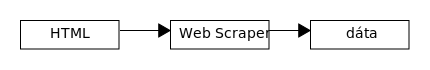
\includegraphics[width= 0.9\textwidth]{diag.png}
    \caption{Princíp extrakcie}
    \label{f:diagram}
\end{figure*}

Na začiatku procesu musíme poznať cieľovú stránku z ktorej chceme dáta získať. Následne potrebujeme získať HTML kód stránky (napríklad pomocou knižnice Requests~\ref{kniznice}). HTML kód využíva tagy ako sú napríklad: h1, div, span. Súčasťou týchto tagov je aj parameter trieda, ktorý odkazuje väčšinou na grafické úpravy tohoto tagu. Pre lepšiu predstavu sú tieto tagy zobrazené na Obr.~\ref{f:html} zo stránky\footnote{\url{https://www.alza.sk/iphone-15-pro-max?dq=7927773}}. Ak by sme v tomto prípade chceli zistiť cenu výrobku, hľadali by sme podľa tagu \textless~span class="price-box\_\_price"\textgreater~. Na vyhľadanie tagu sa použije niektorá z knižníc na extrakciu tagu. Tieto knižnice vyhľadávajú v HTML podľa tagov\cite{9215357}. Výstupom knižnice je nami požadovaný tag s ktorým môžeme ďalej pracovať. Môžeme ho uložiť na neskoršiu analýzu. Výstup z ukážkového HTML by bol "1 449 \EURdig~".

\begin{figure*}[tbh]
    \centering
    \includegraphics[width= 0.9\textwidth]{html.png}
    \caption{Ukážka HTML tagu spolu s triedou}
    \label{f:html}
\end{figure*}


%\cite{10145369} Web Scraping for Data Analytics: A BeautifulSoup Implementation
%\cite{10250745} An Extensive Review on Web Scraping Technique using Python
%\cite{8822022} Data Analysis by Web Scraping using Python
%\cite{9215357} A Survey on Python Libraries Used for Social Media Content Scraping

\section{Príklady reálneho využitia}\label{usecase}
V tejto časti by sme chceli priblížiť niektoré z projektov, ktoré extrahujú dáta z web stránok pomocou Python.

Jedným z príkladov je článok "Phishing Web Page Detection using web Scraping“ \cite{10115148}, v ktorom sa zaoberajú automatizovaným odhaľovaním phishing stránok. Ich riešenie na odhaľovanie takýchto stánok má presnosť detekcie viac ako 98\%. Pri tomto projekte bol požitý Python a knižnica Beautiful Soup(časť~\ref{kniznice}).

Ďalším z príkladov je článok "Food Genie, Recipe Search Algorithm using Web Scraping"\cite{10270597}, ktorý využíva web scraping na porovnanie indegriencíi, ktoré majú ísť do rovnakého receptu. Rieši problém toho že naprieč rôznymi stránkami má recept iný postup alebo sú použité iné suroviny. Napríklad pri tomto projekte bol využitý Python a knižnica scrapy(časť~\ref{kniznice}).

Ako ďalší je článok "Web Scraping Methods on Odoo Framework to Collect Rupiah Exchange Rate From B ank Indonesia Website"\cite{9790917}, ktorý sledoval kurz cudzej meny voči Indonézskej rupie. Pri tomto projekte sa využíva Python a knižnica Beautiful Soup(časť~\ref{kniznice}).

Ako posledný príklad by sme uviedli článok "NEWSONE- AN AGGREGATION SYSTEM FOR NEWS USING WEB SCRAPING METHOD"\cite{8067594}, ktorý požíva web scraping na extrakciu správ z rôznych web stránok v rôznych jazykoch a sústreďuje ich na platformu "NewsOne". Pri tomto projekte sa taktiež využíva Python a knižnica Beautiful Soup(časť~\ref{kniznice}).

Z príkladov je vidieť že Web scraping je využívaný oblastiach ako ekonomika, novinárstvo ale i v gastronómii.

\section{Knižnice pre získavanie dát} \label{kniznice}
Zoznam knižníc, ktoré môžu byť použité na extrakciu dát z webu pre programovací jazyk Python:
\begin{itemize}
\item Requests\footnote{\url{https://pypi.org/project/requests/}} je jednoduchá knižnica ktorá umožňuje vytvoriť http alebo https požiadavky pomocou metódy POST a GET. Táto knižnica je najčastejšie používaná na získanie samotného HTML kódu zo stánky. Ak by sme chceli použiť len samotnú knižnicu museli by sme si na vyhľadávanie napísať vlastný algoritmus. To by bolo zbytočné, pretože existuje niekoľko knižníc, ktoré už obsahujú túto funkcionalitu a sú uvedené nižšie.
\item Beautiful Soup\footnote{\url{https://pypi.org/project/beautifulsoup4/}} táto knižnica obsahuje nástroje na vyhľadávanie, upravovanie a iteráciu v HTML alebo XML kóde. Podmienkou pre fungovanie je vstup vo formáte HTML alebo XML a pre ten sa najčastejšie využíva vyššie spomenutá knižnica Requests.
\item Scrapy\footnote{\url{https://pypi.org/project/Scrapy/}} je rýchly framework pre prehľadávanie webu na vysokej úrovni, ktorý sa používa na prehľadávanie webových stránok a extrahovanie štruktúrovaných údajov. Dá sa použiť na širokú škálu účelov, od získavania dát až po monitorovanie a automatizované testovanie. Výhodou oproti ostatným knižniciam je že obsahuje nástroj na extrakciou HTML kódu zo stránky.
\item Selenium\footnote{\url{https://pypi.org/project/selenium/}} je knižnica, ktorá umožňuje priamo pomocou prehliadača interagovať so stránkami. Podporované prehliadače: Firefox, Chrome, Internet Explorer. V základe je to script, ktorý sa vykonáva v internetovom prehliadači. Keďže sa jedná priamo o prehliadač dokáže uchovávať súbory cookies a taktiež podporuje JavaScript. %pomocou scrit
\item MechanicalSoup\footnote{\url{https://pypi.org/project/MechanicalSoup/}} je knižnica na automatizáciu interakcie s webovými stránkami. MechanicalSoup automaticky ukladá a odosiela súbory cookie, sleduje presmerovania a môže sledovať odkazy a odosielať formuláre. Avšak nepodporuje JavaScript.
\end{itemize}

Toto boli najpoužívanejšie knižnice na extrakciu dát z web stránok. Všetky uvedené knižnice sú zadarmo a Open-source.

\section{Jednoduchý príklad požitím knižnice Beautiful Soup} \label{imp}
\subsection{Kód}
\begin{figure*}[tbh]
    \centering
    \includegraphics[width= 0.9\textwidth]{code.png}
    \caption{Program (výstup: Google)}
    \label{f:code}
\end{figure*}

Na Obr.~\ref{f:code} je príklad kódu, ktorý zo stránky \url{https://www.google.com/} extrahuje názov stánky a teda tag \textless title\textgreater~. Ako prvé sa spraví požiadavka pomocou knižnice Requests, ktorá vráti kód web stránky vo formáte HTML. Na HTML sa použije knižnica Beautiful Soup, ktorá vie pracovať s jednotlivými tagmi v HTML kóde. Knižnici dáme požiadavkou na vypísanie názvu stránky v reťazci. Následne dostaneme výstup "Google". Tento princíp je uvedený v Obr.~\ref{f:diagram}. Podobný postup sa dá využiť aj napríklad na sledovanie ceny produktu a to tak že nájdeme html tag, ktorý obsahuje symbol meny a teda aj číselnú hodnotu.

\subsection{Časová náročnosť}
% časy: https://youtu.be/FQPaAToHJY8
V tejto časti si priblížime množstvo času, ktorý je potrebný na splnenie rovnakej úlohy pomocou knižnice Beautiful Soup a človeka.
\begin{table}[tbh]
    \caption{Porovnanie času pri výpise knižnicou a človekom}
    \includegraphics[width= 1\textwidth]{tab.png}
    \label{f:tab}
\end{table}
Z tabuľky~\ref{f:tab} vyplýva že spracovanie tejto požiadavky teda vypísanie názvu stránky je v priemere o rýchlejšie asi 100-krát.

Pri tejto ukážke sme zaznamenali len čas extrakcie tagu \textless title\textgreater~.

\section{Záver} \label{zaver} % prípadne iný variant názvu
Výsledkom našej práce je článok ktorý približuje tému extrakcie informácii z webu pomocou programovacieho jazyka Python. Vysvetľuje základný princíp web scrapingu a taktiež ukazuje na aktuálnosť tejto témy. Boli vymenované najznámejšie knižnice, ktoré umožňujú efektívne prehliadanie HTML web stránok. Ďalej bol uvedený jednoduchý príklad použitím knižnice Beautiful Soup, ktorý ukazuje rýchlosť a ľahkosť naučenia sa tejto knižnice. Verím že tento článok by mohol byť dobrým úvodom do problematiky extrakcie dát z webu aj s príkladmi. Článok je taktiež semestrálna práca na predmet Metódy inžinierskej prace.

\section{Reakcia na témy z prednášok} \label{reakcia}
\paragraph{Spoločenské súvislosti.}\label{spoloc}
V aktuálnej dobe pri rýchlom rozvoji tento proces tvorí základ získavania dát pre učenie umelej inteligencie. Najznámejšia umelá inteligencia ChatGPT\footnote{\url{ https://chat.openai.com }} využíva tento proces na extrakciu človekom napísaným textov napríklad z online fór\cite{openaiWhatChatGPT}.

\paragraph{Technológia a ľudia.}
Technológia slúži na uľahčenie života ľudom. V súvislosti s našim článkom priamo i nepriamo uľahčuje ľudom život. Nepriamo napríklad vo forme umelej inteligencie. Pri tvorbe modelu pre umelú inteligenciu museli byť použité dáta z web stránok. A priamo tým že ľudia nemusia zložito prepisovať alebo kopírovať údaje zo stránky ale jednoduchým programom môžu získať rovnaké informácie za kratší čas. Asi jedinou zápornou stránkou je že nástupom tejto technológie určite zanikli niektoré pracovné pozície.

\paragraph{Udržateľnosť a etika.}
Udržateľnosť tejto technológie je veľmi dôležitá v dnešnej dobre pri rýchlom rozvoji umelej inteligencie, pretože potrebujeme získavať veľké množstvo dát v krátkom čase. Internet a celkovo web stránky predstavujú najrýchlejší spôsob získavania informácii. Každý deň ho využíva veľký počet pravidelných používateľov.
Tento spôsob získavania informácii môže byt neetický, pretože stránka môže predávať svoje dáta za peniaze a tak obchádzame túto peňažnú bariéru. Týmto problémom sa zaoberajú mnohý ľudia a jedným z príkladov je článok\cite{10092327}, ktorý navrhuje rôzne spôsoby ako zabrániť extrakcii dát. Napríklad používaním Captcha alebo registrovaním sa. Niektoré stránky používajú obmedzenie počtu návštev v určitom čase.

% týmto sa generuje zoznam literatúry z obsahu súboru literatura.bib podľa toho, na čo sa v článku odkazujete
\bibliography{literatura}
\bibliographystyle{plain} % prípadne alpha, abbrv alebo hociktorý iný
\end{document}
